\begin{frame}
  \frametitle{Versuchsaufbau- und durchführung}
\begin{figure}
  \centering
  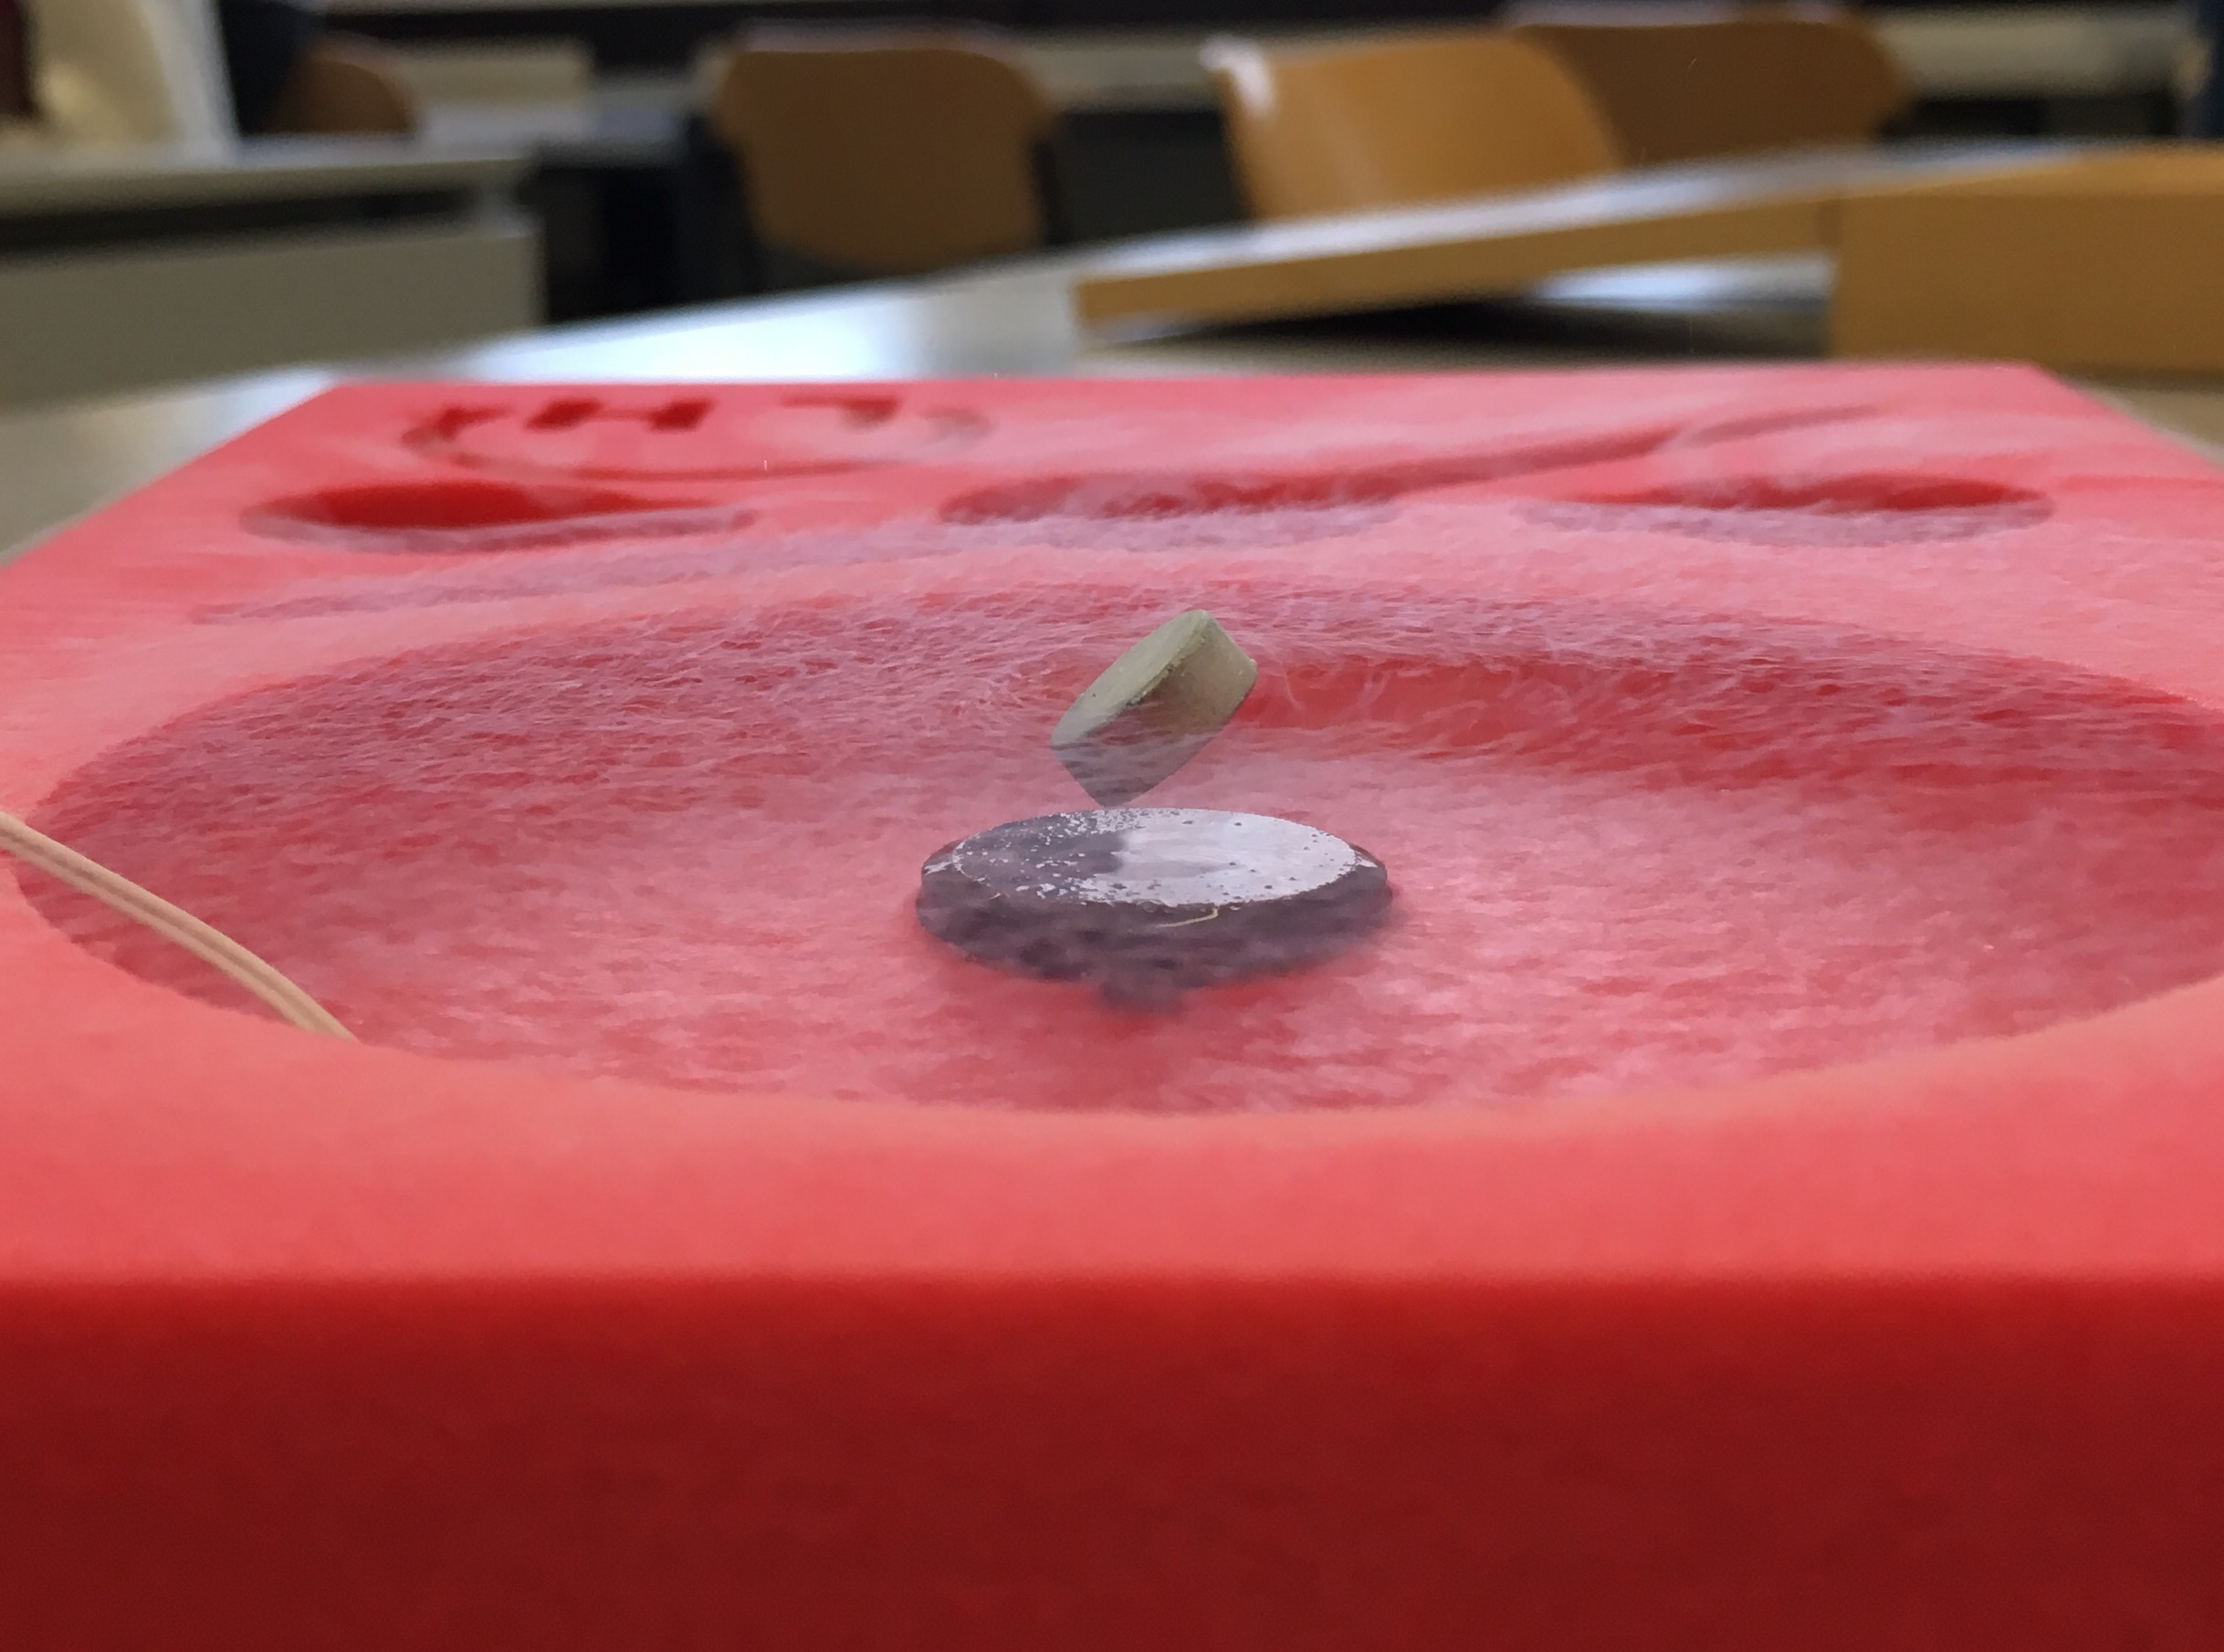
\includegraphics[width=0.7\textwidth]{bilder/versuchsaufbau.jpg}
  \label{fig: versuchsaufbau}
\end{figure}
\end{frame}

\begin{frame}
  \frametitle{Auswertung der kritischen Temperatur}
\begin{columns}
  \begin{column}{0.5\textwidth}
  \begin{tabular}{SSS}
  \toprule
  {Messwert} & {Spannung in $\si{\milli\volt}$}  &  {Temperatur in $\si{\celsius}$}  \\
  \midrule
   1  & -5.70  & -192.68\\
  2  & -5.77  & -195.00\\
  3  & -5.77  & -195.00\\
  4  & -5.76  & -194.67\\
  5  & -5.76  & -194.67\\
  6  & -5.75 & -194.34\\
  7  & -5.76 & -194.67\\
  8  & -5.76  & -194.67\\
  9  & -5.75  & -194.34\\

  \bottomrule
  \end{tabular}
\end{column}

\begin{column}{0.5\textwidth}
\begin{equation*}
  T_{\mathrm{mittel}}=\SI{-194.5\pm0.7}{\celsius}
\end{equation*}
\begin{equation*}
  \Delta T= \SI{14.5\pm0.7}{\celsius} \quad (-7\%)
\end{equation*}
\end{column}
\end{columns}

\end{frame}
